\newcommand{\baselineAlgorithm}{%
\begin{algorithm}
\SetAlgoLined
$i = 0$\;
\lnl{loop} \While{i $<$ d}{
$l = h_i(ikey)$\;
\uIf{$key_l = ikey$}{$val_l$++; end\;}
\uElseIf{$val_l = 0$}{l = (ikey, 1); end\;}
\Else{$min = update(min)$\;}
$i$++\;
}
\uIf{$i = d$}{$min = (ikey, val_{min} + 1)$\;}
\end{algorithm}}

\newcommand{\OurAlgorithm}{%
\begin{algorithm}
\SetAlgoLined
$i = 0, cKey = iKey, cVal = 1$\;
\lnl{loop} \While{i $<$ d}{
$l = h_i(cKey)$\;
\uIf{$key_l = ckey$}{$val_l$ += $cVal$; end\;}
\uElseIf{$val_l = 0$}{l = (ckey, cVal); end\;}
\uElseIf{$val_l < cVal$}{swap $(key_l, val_l)$ with $(cKey, cVal)$\;}
$i$++\;
}
\end{algorithm}}

\section{HashPipe based Heavy Hitter Algorithm}\label{sec:algorithm} 

As described in \Sec{sec:related}, \TheSystem is heavily inspired by the \spacesaving algorithm \cite{metwally2005efficient}, which we describe now
(\Sec{sec:spacesaving}). In the later subsections
(\Sec{sec:sampling-d}-\Sec{sec:feed-forward}), we describe our modifications to
the algorithm to make it amenable to switch implementation.
%

\subsection{\spacesaving\ Algorithm}
\label{sec:spacesaving}

To track the $k$ heaviest items, \spacesaving uses a table with $m$ (which is
$O(k)$) slots, each of which identifies a distinct flow key and its counter. All
slots are initially empty, \ie keys and counters are set to zero.

\begin{algorithm}
\DontPrintSemicolon % Some LaTeX compilers require you to use
% \dontprintsemicolon instead
\Comment{Table $T$ has $m$ slots, either containing $(key_j, val_j)$ at slot $j
  \in \{1, \ldots, m\}$, or empty. Incoming packet has key $iKey$.}\;

\eIf{$\exists$ slot $j$ in $T$ with $iKey = key_j$}{
  $val_j \gets val_j + 1$\;
}{
  \eIf{$\exists$ empty slot $j$ in $T$}{
    $(key_j, val_j) \gets (iKey, 1)$\;
  }{
    $m \gets argmin_{j \in \{1,\ldots,m\}}(val_j)$\;\label{alg:ss:minfind}
    $(key_m, val_m) \gets (iKey, val_m+1)$\;
  }
}
%% $min \gets 1$\;
%% \For{$i \gets 2$ \textbf{to} $m$} {
%%   \If{$val_i < val_{min}$} {
%%     $min \gets i$\;
%%   }
%% }
%% $min \gets (iKey, val_{min} + 1)$\;
\caption{\spacesaving algorithm~\cite{metwally2005efficient}}
\label{algo:spacesaving}
\end{algorithm}

The algorithm is summarized in \Alg{spacesaving}.\footnote{We show the algorithm
  for packet counting; it easily generalizes to byte counts.}
%
When a packet arrives, if its corresponding flow isn't already in the table, and
there is space left in the table, \spacesaving inserts the new flow with a count
of 1. If the flow is present in the table, the algorithm updates the
corresponding flow counter. However, if the table is full, and the flow isn't
found in the table, the algorithm replaces the flow entry that has the {\em
  minimum} counter value in the table with the incoming packet's flow, and
increments this minimum-valued counter.

This algorithm has three useful accuracy properties~\cite{metwally2005efficient}
that we list here. Suppose the true count of flow $key_j$ is $c_j$, and its
count in the table is $val_j$. First, no flow counter in the table is ever
underestimated, \ie $val_j \geq c_j$.
%%  since counters are never
%% decremented and consequently, the minimum is increasing.
Second, the minimum value in the table $val_m$ is an upper bound on the
overestimation error of any counter, \ie $val_j \leq c_j + val_m$.
%% This is because when a flow's counter is initialized with $val_m + 1$, its
%% value is overestimated by at most $val_m$ (if it was a brand new flow that
%% should have otherwise had a counter value $1$).
Finally, any flow with true count higher than the average table count, \ie $c_j
> C/m$, will always be present in the table (here $C$ is the total packet count
added into the table). This last error guarantee is particularly useful for the
threshold-heavy-hitter problem (\Sec{sec:problem}), since by using $1/t$
counters, we can extract all flows whose true count exceeds a threshold $t$ of
the total count. However, this guarantee cannot be extended directly to the
top-$k$ problem, since due to the heavy-tailed nature of
traffic~\cite{estan2002new}, the $k$th heaviest flow contributes nowhere close
to $1/k$th of total traffic.

However, the algorithm step of finding the minimum counter in the table (line
\ref{alg:ss:minfind})---possibly for each packet---is difficult within switch
hardware constraints (\Sec{sec:related}).
%
In the following subsections, we discuss how we incrementally modify the
\spacesaving algorithm to run on hardware switches.

%% While this seems like the best way to approach this problem, this is not
%% feasible in practice since it needs one to examine the entire list (entries in
%% the form of a table) which is not feasible at line-rate. Alternatively, one
%% could use a sorted data structure like a heap that would maintain the
%% minimum. However, complex data structures like heaps or sorted lists do not
%% involve deterministically O(1) cost per packet since once in a while, the
%% compression process for preserving order could involve an O(k) operation. Hence,
%% we need a different version amenable on hardware. \jrex{nice paragraph but very
%%   terse if readers haven't seen these algorithms before. also, in the
%%   pseudocode, min is sometimes a single number and sometimes a tuple}

\subsection{Sampling for the Minimum Value}
\label{sec:sampling-d}

The first simplification we make is to look at the minimum of a small, {\em
  constant} number $d$ of randomly chosen counters, instead of the entire table
(in line \ref{alg:ss:minfind}, \Alg{spacesaving}). This restricts the worst-case
number of memory accesses per packet to a small fixed constant $d$.  The
modified version, \Baseline, is shown in \Alg{Baseline}. The main change from
\Alg{spacesaving} is in the set of table slots examined (while looking up or
updating any key), which is now a set of $d$ slots obtained by hashing the
incoming key using $d$ independent hash functions.

In effect, we {\em sample} the table to estimate a minimum using a few
locations. However, the minimum of just $d$ slots can be far from the minimum of
the entire table of $m$ slots. An inflated value of the minimum could impact the
useful error guarantees of \spacesaving (\Sec{sec:spacesaving}). However, we
show analytically that the overestimation error is not too far from the average
table count $C/m$ with high probability. Further, our
evaluations in \Sec{subsec:comparisonIdeal} show that the distributions of the
minimum of the entire table and of the subsample are comparable.

%% In order to determine the minimum among the entries of a hash table, one would
%% usually need to scan all the complete set of key-value pairs. However, given
%% that that is not feasible, and that only reading a small constant number of
%% locations would be feasible, we attempt to approximate the minimum by reading
%% these locations alone and finding the minimum among them. Section
%% \ignore{include eval} shows that this process of approximating the minimum
%% results in an approximation that is reasonably close to the minimum of the
%% entire table. Independent hash functions are used to pick the indices from where
%% the values would be read to approximate the minimum.

%% the switch to generate multiple indices
%% in the same table by hashing on the incoming flow with $d$ different hash
%% functions. Further,

However, \Alg{Baseline} still requires the switch to read $d$ locations at once
to determine their minimum, and then write back the updated value. This
necessitates a read-modify-write operation, involving $d$ reads and one write
{\em anywhere in table memory}, within the per-packet time budget. However,
multiple reads to the same table ($d > 1$) are supported neither in switch
programming languages today~\cite{bosshart2014p4} nor in emerging programmable
switching chips~\cite{RMT}. Further, supporting multiple reads for every packet
at line rate requires multiported memories with strict access-latency
guarantees, which can be quite expensive in terms of area and
power~\cite{cmos-vlsi-design-book, vlsi-memory-lecture}.

\subsection{Multiple Stages of Hash Tables}
\label{sec:multiple-stages-d}
The next step is to reduce the number of reads to memory to facilitate operation
at line rate. We split the counter table $T$ into $d$ disjoint tables, and we
read exactly one slot per table. The algorithm is exactly the same as
\Alg{Baseline}; except that now hash function $h_i$ returns only slots in the
$i$th stage.

This design enables pipelining the memory accesses to the $d$ tables, since
different packets can access different tables at the same time. However, packets
may need to make two passes through this pipeline: once to determine the counter
with the minimum value among $d$ slots, and a second time to update that
counter. The second pass is possible through ``recirculation'' of packets
through the switching pipeline~\cite{p4-v1.1-spec, ovs-packet-recirculation,
  arista-7050-datasheet} with additional metadata on the packet, allowing the
switch to increment the minimum-valued counter in the second pass. However, the
second pass is potentially needed for {\em every packet}, and recirculating
every packet can halve the pipeline bandwidth available to process packets.

%% We essentially use $d$ different hash functions on the incoming flow’s key, one
%% per stage to pick exactly one location amongst the entries per stage. In this
%% manner, we are able to reduce the number of reads to one per-stage and carry
%% over the read values as metadata. The computation of the minimum can be done
%% using this state carried over at the end of the processing pipeline. However, if
%% the location where the new flow is to be rewritten is anything other than the
%% last stage, this would pose a problem. The feed-forward \ignore{cite}
%% restriction implies that a packet cannot make modifications to earlier stages in
%% the pipeline once it has passed through them. Hence, if this model was to work,
%% the packet would need to be recirculated into the pipeline and all incoming
%% packets would have to be stalled until the current packet finishes modification
%% to the appropriate pipelined stage. Clearly, this wouldn’t be feasible at line
%% rate where each stage processes a packet independently and atomically in a
%% pipelined fashion to speed up processing.

\begin{algorithm}
\DontPrintSemicolon % Some LaTeX compilers require you to use \dontprintsemicolon instead
%\KwIn{A finite set $A=\{a_1, a_2, \ldots, a_n\}$ of integers}
%\KwOut{The largest element in the set}
\Comment{Hash functions $h_i(iKey) \rightarrow$ slots, $i \in \{1,\dots,d\}$}\;

%% \For{$i \gets 1 $ \textbf{to} $d$} {
%% $l \gets h_i(ikey)$\;
%%   \If{$key_l = iKey$} {
%%     $val_l \gets val_l + 1$;\;
%%   }
%%   \ElseIf{$val_l = 0$}{
%%   	$(key_l,val_l) \gets (iKey, 1)$;\;
%%   }
%%   \Else{
%%   	$minLoc = update(minLoc)$
%%   }
%% }
%% \If{$i > d$}{$ minLoc \gets (ikey, val_{minLoc} + 1)$\;}

$H = \{h_1(iKey), \ldots, h_d(iKey)\}$\;
\eIf{$\exists$ slot $j \in H$ with $iKey = key_j$}{
  $val_j \gets val_j + 1$\;
}{
  \eIf{$\exists$ empty slot $j \in H$}{
    $(key_j, val_j) \gets (iKey, 1)$\;
  }{
    $m \gets argmin_{j \in H}(val_j)$\;\label{alg:hp:minfind}
    $(key_m, val_m) \gets (iKey, val_m+1)$\;
  }
}

\caption{\Baseline: Sample $d$ slots at once}
\label{algo:Baseline}
\end{algorithm}

\subsection{Feed-Forward Packet Processing}
\label{sec:feed-forward}
We now alleviate the need to process a packet more than once through the switch
pipeline, using two key ideas.

\begin{figure*}[h] 
  \begin{subfigure}[b]{0.45\linewidth}
    \centering
    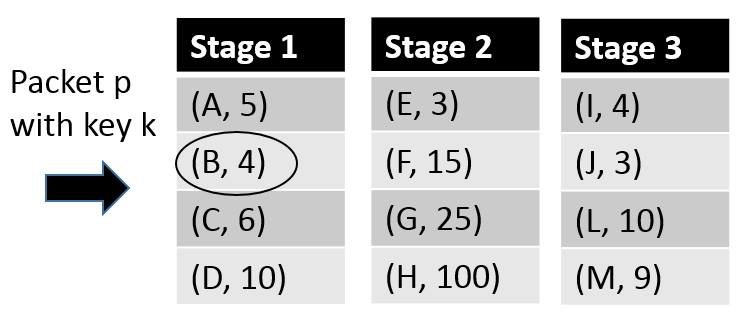
\includegraphics[width=0.75\linewidth, height=2.5cm]{entry.png} 
    \caption{Initial status of table} 
    \label{alg:a} 
    \vspace{4ex}
  \end{subfigure}%% 
  \begin{subfigure}[b]{0.45\linewidth}
    \centering
    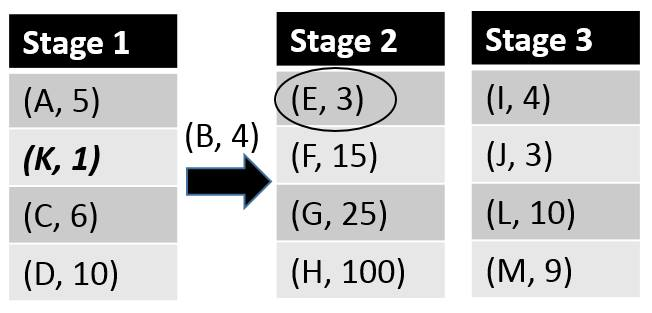
\includegraphics[width=0.75\linewidth, height=2.5cm]{2nd_stage.png} 
    \caption{New flow is placed with value $1$ in first stage of table} 
    \label{alg:b} 
    \vspace{4ex}
  \end{subfigure} 
  \begin{subfigure}[b]{0.45\linewidth}
    \centering
    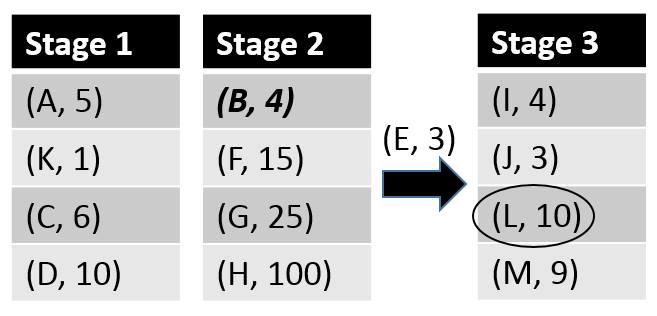
\includegraphics[width=0.75\linewidth, height=2.5cm]{3rd_stage.png} 
    \caption{$B$ being larger evicts $E$} 
    \label{alg:c} 
  \end{subfigure}%%
  \begin{subfigure}[b]{0.45\linewidth}
    \centering
    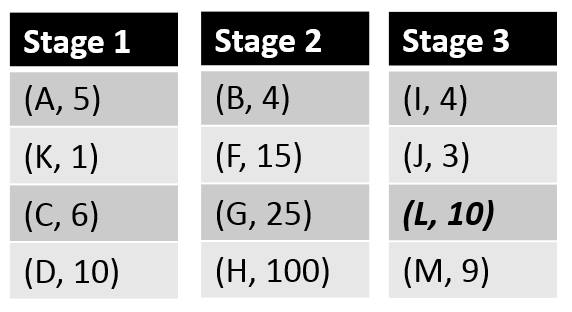
\includegraphics[width=0.75\linewidth, height=2.5cm]{final_stage.png} 
    \caption{$L$ being larger is retained in the table} 
    \label{alg:d} 
  \end{subfigure} 
  \\
  \caption{An illustration of \TheSystem.}
  \label{fig:HashPipe} 
\end{figure*}

\NewPara{Track a rolling minimum.} We track the minimum counter value seen so
far (and its key) as the packet traverses the pipeline, by {\em moving} the
counter and key through the pipeline as {\em packet metadata.} Emerging
programmable switches allow the use of such metadata to communicate results of
packet processing between different stages, and such metadata can be written to
at any stage, and used for packet matching at a later stage~\cite{p4-v1.1-spec}.

\begin{algorithm}
\DontPrintSemicolon % Some LaTeX compilers require you to use \dontprintsemicolon instead
%\KwIn{A finite set $A=\{a_1, a_2, \ldots, a_n\}$ of integers}
%\KwOut{The largest element in the set}
\Comment{Insert in the first stage}\;
$l_1 \gets h_1(iKey)$\;
\If{$key_{l_1} = iKey$}{
  $val_{l_1} \gets val_{l_1} + 1$\;
  end processing\;
}\ElseIf{$l_1$ is an empty slot}{
  $(key_{l_1}, val_{l_1}) \gets (iKey, 1)$\;
  end processing\;
}\Else{
  $(cKey, cVal) \gets (key_{l_1}, val_{l_1})$\;
  $(key_{l_1}, val_{l_1}) \gets (iKey, 1)$\;
}
\Comment{Track a rolling minimum}\;
\For{$i \gets 2$ \textbf{to} $d$} {
$l \gets h_i(cKey)$\;
  \If{$key_l = cKey$} {
    $val_l \gets val_l + cVal$\;
    end processing\;
  }
  \ElseIf{$l$ is an empty slot}{
    $(key_l, val_l) \gets (cKey, CVal)$\;
    end processing\;
  }
  \ElseIf{$val_l < cVal$}{
    swap $(cKey, cVal)$ with $(key_l, val_l)$
  }
}
\caption{\TheSystem: Pipeline of $d$ hash tables}
\label{algo:Sequential}
\end{algorithm}

As the packet moves through the pipeline, the switch hashes into each stage on
the {\em carried key,} instead of hashing on the key corresponding to the
incoming packet. If the keys match in the table, or the slot is empty, the
counter is updated in the usual way, and the key need no longer be carried
forward with the packet. Otherwise, the keys and counts corresponding to the
{\em larger} of the counters that is carried and the one in the slot is written
back into the table, and the smaller of the two is carried on the packet. We
leverage arithmetic and logical action operations available in the match-action
tables in emerging switches~\cite{RMT} to implement the counter comparison. The
key may be carried to the next stage, or evicted completely from the tables when
the packet reaches the last (\ie $d$th) stage.

\NewPara{Always insert in the first stage.} If the incoming key isn't found in
the first stage in the pipeline, there is no associated counter value to compare
with the key that is in that table. Here, we choose to {\em always insert the
  new flow} in the first stage, and evict the existing key and counter into
packet metadata. After this stage, the packet can track the rolling minimum of
the {\em subsequent stages} in the usual way described above. The final
algorithm, \TheSystem, is shown in \Alg{Sequential}.

One consequence of always inserting an incoming key in the first stage is the
possibility of duplicate keys across different tables in the pipeline, since the
key can exist at a later stage in the pipeline. Note that this is unavoidable
when packets only move once through the pipeline. It is possible that such
duplicates may occupy space in the table, leaving fewer slots for heavy flows,
and causing evictions of heavy flows whose counts may be split across the
duplicate entries.

\label{sec:coalescing}
However, many of these duplicates are easily {\em merged} through the algorithm
itself, \ie the minimum tracking merges counters when the carried key has a
``hit'' in the table. Further, switches can easily estimate the flow count
corresponding to any packet in the data plane itself by summing all the matching
flow counters; so can a data collector, after reading the tables out of the
switch. We also show in our evaluations (\Sec{subsec:sensitivity}) that
  duplicates only have a small effect on the memory available to heavy keys in the table.

\Fig{HashPipe} illustrates an example of processing a packet using \TheSystem. A
packet with a key $K$ enters the switch pipeline (a), and since it isn't found
in the first table, it is inserted there (b). Key $B$ (that was in the slot
currently occupied by $K$) is carried with the packet to the next stage, where
it hashes to the slot containing key $E$. But since the count of $B$ is larger
than that of $E$, $B$ is written to the table and $E$ is carried out on the
packet instead (c). Finally, since the count of $L$ (that $E$ hashes to) is
larger than that of $E$, $L$ stays in the table (d). The net effect is that the new
key $K$ is inserted in the table, and the minimum of the three keys $B$, $E$, and
$L$---namely $E$---is evicted in its favor.

%% The only way to fix the need for packet recirculation would be to make a local
%% approximation as a packet passes through a particular stage in the packet
%% processing pipeline as to what the minimum across the $d$ stages might be. What
%% this means is that we hash on the incoming flow’s key in the first stage and
%% update its counter if it is present in the corresponding location. If not, we
%% treat it as a new key and insert the flow with value 1 in the first table stage,
%% evicting any other flow that might be present in that location. In all further
%% table stages, we carry a flow with a count as metadata on the packet. This
%% carried flow represents the current minimum as observed upon passing the current
%% table stage.

%% At every table stage, based on the carried flow, its count and the flow and its
%% count in the location that the carried flow hashes to (when hashed using the
%% hash function in this particular stage), we make a local choice in favor of
%% retaining the flow with a heavier count. Of course, if any location that the
%% carried flow hashes to is empty, we place the flow and count there and zero out
%% the packet metadata fields so that they do not affect any subsequent
%% stages. When a packet finishes the entire pipeline, the consequence is that the
%% ultimate flow evicted out of the table is a relative minimum and all
%% intermediate flows are given a chance to be placed again in a future table stage
%% if there are smaller flows in later tables.


%%\subsection{Coalescing Duplicate Keys}


%% The one issue with the above mentioned algorithm is that the incoming flow is
%% placed in the first stage without any knowledge on whether this flows is present
%% at a later table stage or not. To get around this, we ensure that if the key
%% being carried is the same as the key present in the location it hashes to, we
%% coalesce the two values, the carried one with the one present in the table. We
%% also expect the controller to interpret the actual count associated with a flow
%% as the sum of the counts in the multiple occurrences of the flow in the
%% table. We show in our evaluations that despite the presence of duplicates, and
%% increased number of evictions by smaller flows due to the presence of split
%% counts for each flow\ignore{explain more?}, our algorithm performs
%% well\ignore{refer right place}. The final algorithm is detailed in
%% \ignore{refer}.

%\subsection{Baseline Implementation/ All Probes at once}

%Given that we are interested in the top $k$ keys by value or count, the most unlikely candidate would be the key with the least value amongst the keys in the $d$ locations if a given incoming key is competing with $d$ keys at the locations its hashes to across $d$ tables. Hence, the most basic modification of the d-left hashing scheme to determine the heavy hitters involves an update to the existing location if the key is already present or insertion of the new key into the leftmost empty location if there is one or eviction of the key with the least value amongst the $d$ candidate keys. When replacing this minimum entry with the new key, the value assigned to it could be $1$, if treated as a brand new flow or the current minimum value + 1, as done in . This translates to the algorithm in %Fig:~\ref{Basic Implementation}%
%which generically calls the value "newVal". In order to reduce the number of passes through the hash table, the minimum amongst the $d$ locations is found as the algorithm looks for the leftmost empty location or the key itself for a given incoming key. This algorithm is hard to implement in practice though since the collision handling mechanism requires one to go back to a previously traversed table stage after determining the minimum and make a modification to it for a given packet that has already passed through these tables in the packet processing pipeline. This would cause a lot of delay and is very impractical.

%\subsection{Sequential Probes/Feed Forward}

%Since the ultimate goal is to implement the algorithm on hardware and multi-ported reads would involve more combinational circuits, reducing the number of lookups per stage could also be useful. Hence, instead of hashing on both the evicted key from a previous table stage and the original key like the algorithm in Section 6.3, we limit ourselves to hashing only on the evicted key or the key being carried and finding a location for it. However, this approach could leave us with multiple occurences of the same key with different values that we aren't even aware of since we are no longer looking for it and updating those values. However, our simulation show that this is still reasonable, as long as the controller is reading and interpreting these values correctly and associating the sum across the multiple values as the real value associated with a particular key (since the values are split acorss multiple occurences in this case). The algorithm is detailed on the right side of %Fig:~\ref{fig:HardwareImplementable}. 

%The one downside of this approach is that if the value of a key is split between two locations with neither of them individually high enough relative to the values of other keys even though their sum (the actual value associated with that flow) is high enough to make that flow a heavy hitter, the chances of all occurences of that key being evicted are fairly high. The multiple lookup case (Section 6.3), on the other hand, tries to address this by making the values in the later table stages more accurate and hence, more robust to eviction.
